\documentclass[14pt]{extbook}
\usepackage{multicol, enumerate, enumitem, hyperref, color, soul, setspace, parskip, fancyhdr} %General Packages
\usepackage{amssymb, amsthm, amsmath, latexsym, units, mathtools} %Math Packages
\everymath{\displaystyle} %All math in Display Style
% Packages with additional options
\usepackage[headsep=0.5cm,headheight=12pt, left=1 in,right= 1 in,top= 1 in,bottom= 1 in]{geometry}
\usepackage[usenames,dvipsnames]{xcolor}
\usepackage{dashrule}  % Package to use the command below to create lines between items
\newcommand{\litem}[1]{\item#1\hspace*{-1cm}\rule{\textwidth}{0.4pt}}
\pagestyle{fancy}
\lhead{Makeup Progress Quiz 3}
\chead{}
\rhead{Version C}
\lfoot{1648-1753}
\cfoot{}
\rfoot{Summer C 2021}
\begin{document}

\begin{enumerate}
\litem{
Solve the quadratic equation below. Then, choose the intervals that the solutions $x_1$ and $x_2$ belong to, with $x_1 \leq x_2$.\[ 20x^{2} -21 x -54 = 0 \]\begin{enumerate}[label=\Alph*.]
\item \( x_1 \in [-3.85, -3.18] \text{ and } x_2 \in [0.67, 0.88] \)
\item \( x_1 \in [-0.8, 0.96] \text{ and } x_2 \in [4.45, 4.58] \)
\item \( x_1 \in [-1.92, -0.67] \text{ and } x_2 \in [2.06, 2.64] \)
\item \( x_1 \in [-6.22, -5.51] \text{ and } x_2 \in [-0.51, 0.47] \)
\item \( x_1 \in [-24.34, -23.91] \text{ and } x_2 \in [44.99, 45.65] \)

\end{enumerate} }
\litem{
Factor the quadratic below. Then, choose the intervals that contain the constants in the form $(ax+b)(cx+d); b \leq d.$\[ 24x^{2} +38 x + 15 \]\begin{enumerate}[label=\Alph*.]
\item \( a \in [1.28, 2.59], \hspace*{5mm} b \in [3, 10], \hspace*{5mm} c \in [10.63, 14.02], \text{ and } \hspace*{5mm} d \in [5, 8] \)
\item \( a \in [0.84, 1.07], \hspace*{5mm} b \in [13, 23], \hspace*{5mm} c \in [-0.46, 1.61], \text{ and } \hspace*{5mm} d \in [14, 26] \)
\item \( a \in [3.23, 4.62], \hspace*{5mm} b \in [3, 10], \hspace*{5mm} c \in [5.33, 6.32], \text{ and } \hspace*{5mm} d \in [5, 8] \)
\item \( a \in [11.82, 12.46], \hspace*{5mm} b \in [3, 10], \hspace*{5mm} c \in [1.49, 2.68], \text{ and } \hspace*{5mm} d \in [5, 8] \)
\item \( \text{None of the above.} \)

\end{enumerate} }
\litem{
Graph the equation below.\[ f(x) = -(x-2)^2 - 15 \]\begin{enumerate}[label=\Alph*.]
\begin{multicols}{2}\item 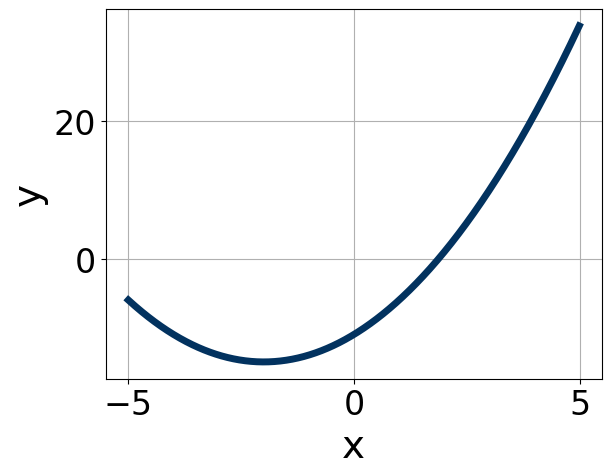
\includegraphics[width = 0.3\textwidth]{../Figures/quadraticEquationToGraphAC.png}\item 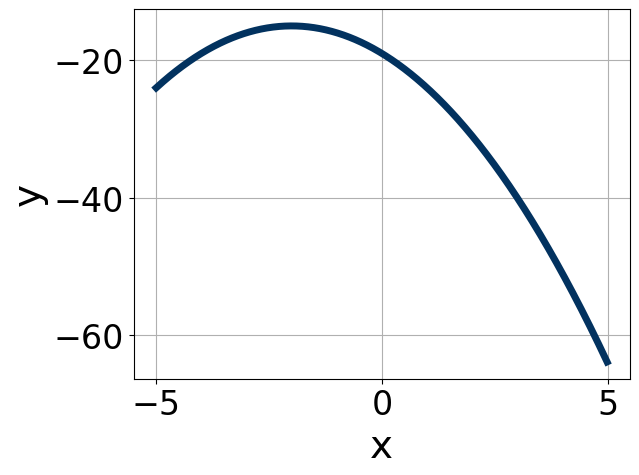
\includegraphics[width = 0.3\textwidth]{../Figures/quadraticEquationToGraphBC.png}\item 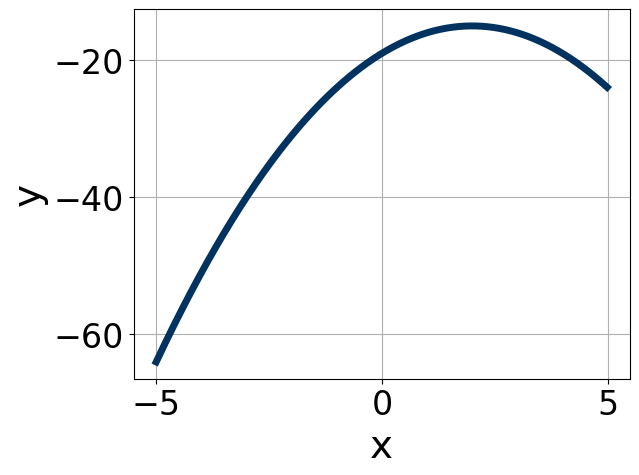
\includegraphics[width = 0.3\textwidth]{../Figures/quadraticEquationToGraphCC.png}\item 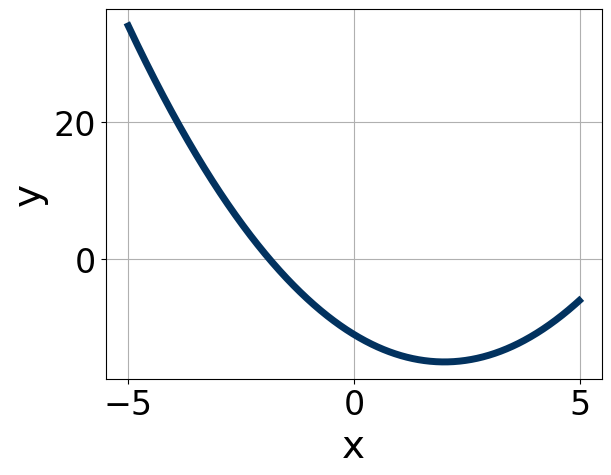
\includegraphics[width = 0.3\textwidth]{../Figures/quadraticEquationToGraphDC.png}\end{multicols}\item None of the above.
\end{enumerate} }
\litem{
Factor the quadratic below. Then, choose the intervals that contain the constants in the form $(ax+b)(cx+d); b \leq d.$\[ 24x^{2} -50 x + 25 \]\begin{enumerate}[label=\Alph*.]
\item \( a \in [2.6, 4.2], \hspace*{5mm} b \in [-6, 2], \hspace*{5mm} c \in [6.24, 8.28], \text{ and } \hspace*{5mm} d \in [-6, 2] \)
\item \( a \in [9.8, 12.2], \hspace*{5mm} b \in [-6, 2], \hspace*{5mm} c \in [1.28, 2.4], \text{ and } \hspace*{5mm} d \in [-6, 2] \)
\item \( a \in [3.4, 6.1], \hspace*{5mm} b \in [-6, 2], \hspace*{5mm} c \in [3.69, 5.33], \text{ and } \hspace*{5mm} d \in [-6, 2] \)
\item \( a \in [-1.5, 2.5], \hspace*{5mm} b \in [-35, -22], \hspace*{5mm} c \in [0.81, 1.48], \text{ and } \hspace*{5mm} d \in [-25, -12] \)
\item \( \text{None of the above.} \)

\end{enumerate} }
\litem{
Write the equation of the graph presented below in the form $f(x)=ax^2+bx+c$, assuming  $a=1$ or $a=-1$. Then, choose the intervals that $a, b,$ and $c$ belong to.
\begin{center}
    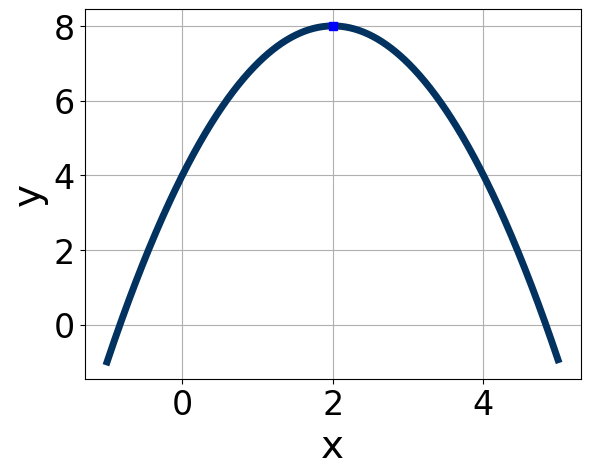
\includegraphics[width=0.5\textwidth]{../Figures/quadraticGraphToEquationCopyC.png}
\end{center}
\begin{enumerate}[label=\Alph*.]
\item \( a \in [-4, 0], \hspace*{5mm} b \in [-6, -1], \text{ and } \hspace*{5mm} c \in [-14, -7] \)
\item \( a \in [1, 5], \hspace*{5mm} b \in [-6, -1], \text{ and } \hspace*{5mm} c \in [12, 17] \)
\item \( a \in [1, 5], \hspace*{5mm} b \in [4, 7], \text{ and } \hspace*{5mm} c \in [12, 17] \)
\item \( a \in [-4, 0], \hspace*{5mm} b \in [4, 7], \text{ and } \hspace*{5mm} c \in [2, 6] \)
\item \( a \in [-4, 0], \hspace*{5mm} b \in [-6, -1], \text{ and } \hspace*{5mm} c \in [2, 6] \)

\end{enumerate} }
\litem{
Solve the quadratic equation below. Then, choose the intervals that the solutions belong to, with $x_1 \leq x_2$ (if they exist).\[ 20x^{2} -12 x -5 = 0 \]\begin{enumerate}[label=\Alph*.]
\item \( x_1 \in [-0.94, -0.61] \text{ and } x_2 \in [-0.1, 0.7] \)
\item \( x_1 \in [-6.24, -5.08] \text{ and } x_2 \in [16.6, 19.4] \)
\item \( x_1 \in [-0.68, 0.72] \text{ and } x_2 \in [0.3, 1.4] \)
\item \( x_1 \in [-23.25, -22.33] \text{ and } x_2 \in [22.7, 24.8] \)
\item \( \text{There are no Real solutions.} \)

\end{enumerate} }
\litem{
Solve the quadratic equation below. Then, choose the intervals that the solutions belong to, with $x_1 \leq x_2$ (if they exist).\[ 16x^{2} +10 x -7 = 0 \]\begin{enumerate}[label=\Alph*.]
\item \( x_1 \in [-1.9, -0.86] \text{ and } x_2 \in [-0.33, 0.66] \)
\item \( x_1 \in [-0.86, 0.5] \text{ and } x_2 \in [0.78, 1.2] \)
\item \( x_1 \in [-17.2, -15.65] \text{ and } x_2 \in [6.61, 6.82] \)
\item \( x_1 \in [-24.09, -23.27] \text{ and } x_2 \in [23, 23.38] \)
\item \( \text{There are no Real solutions.} \)

\end{enumerate} }
\litem{
Solve the quadratic equation below. Then, choose the intervals that the solutions $x_1$ and $x_2$ belong to, with $x_1 \leq x_2$.\[ 10x^{2} -57 x + 54 = 0 \]\begin{enumerate}[label=\Alph*.]
\item \( x_1 \in [1, 1.28] \text{ and } x_2 \in [4.16, 4.76] \)
\item \( x_1 \in [11.78, 12.58] \text{ and } x_2 \in [43.2, 46.27] \)
\item \( x_1 \in [0.69, 0.93] \text{ and } x_2 \in [4.66, 6.35] \)
\item \( x_1 \in [1.44, 1.56] \text{ and } x_2 \in [2.77, 3.98] \)
\item \( x_1 \in [0.45, 0.71] \text{ and } x_2 \in [7.78, 10.35] \)

\end{enumerate} }
\litem{
Write the equation of the graph presented below in the form $f(x)=ax^2+bx+c$, assuming  $a=1$ or $a=-1$. Then, choose the intervals that $a, b,$ and $c$ belong to.
\begin{center}
    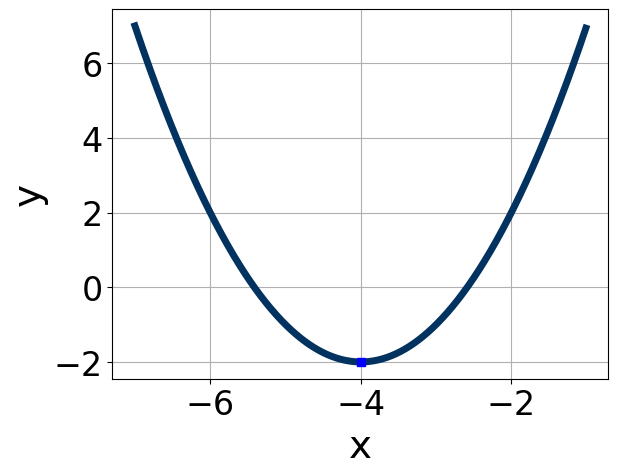
\includegraphics[width=0.5\textwidth]{../Figures/quadraticGraphToEquationC.png}
\end{center}
\begin{enumerate}[label=\Alph*.]
\item \( a \in [0.3, 1.4], \hspace*{5mm} b \in [-8, -4], \text{ and } \hspace*{5mm} c \in [13, 17] \)
\item \( a \in [0.3, 1.4], \hspace*{5mm} b \in [-8, -4], \text{ and } \hspace*{5mm} c \in [17, 19] \)
\item \( a \in [-1.7, -0.4], \hspace*{5mm} b \in [-8, -4], \text{ and } \hspace*{5mm} c \in [-20, -15] \)
\item \( a \in [-1.7, -0.4], \hspace*{5mm} b \in [6, 10], \text{ and } \hspace*{5mm} c \in [-20, -15] \)
\item \( a \in [0.3, 1.4], \hspace*{5mm} b \in [6, 10], \text{ and } \hspace*{5mm} c \in [13, 17] \)

\end{enumerate} }
\litem{
Graph the equation below.\[ f(x) = -(x+3)^2 - 15 \]\begin{enumerate}[label=\Alph*.]
\begin{multicols}{2}\item 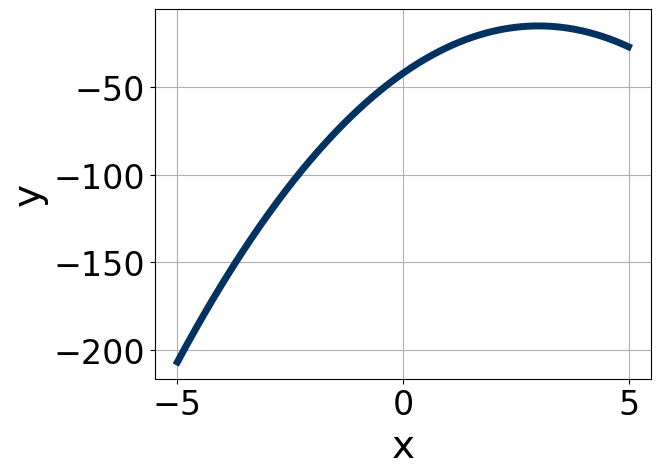
\includegraphics[width = 0.3\textwidth]{../Figures/quadraticEquationToGraphCopyAC.png}\item 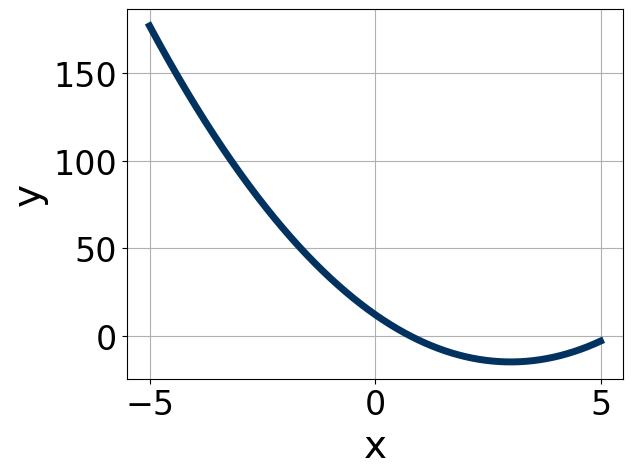
\includegraphics[width = 0.3\textwidth]{../Figures/quadraticEquationToGraphCopyBC.png}\item 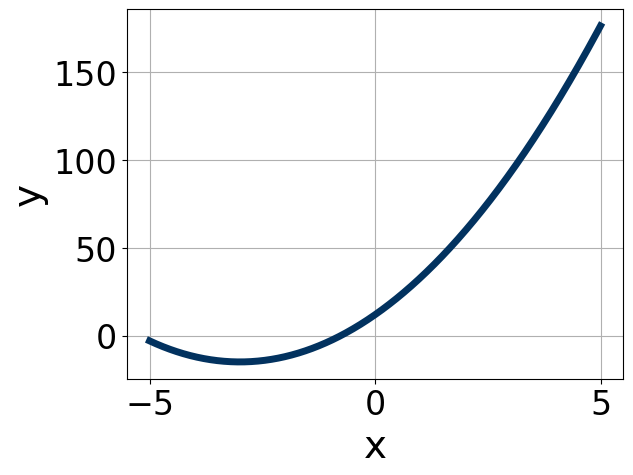
\includegraphics[width = 0.3\textwidth]{../Figures/quadraticEquationToGraphCopyCC.png}\item 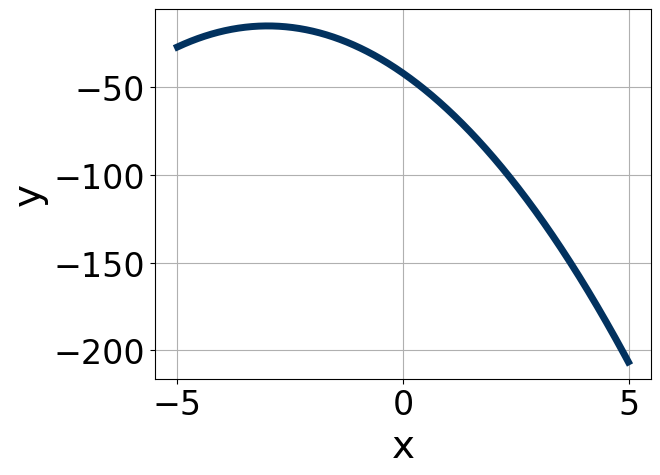
\includegraphics[width = 0.3\textwidth]{../Figures/quadraticEquationToGraphCopyDC.png}\end{multicols}\item None of the above.
\end{enumerate} }
\end{enumerate}

\end{document}